\documentclass[xcolor=table]{beamer}
\usepackage[utf8]{inputenc}
\usepackage[T1]{fontenc} 
\usepackage[english]{babel} 
\usepackage{graphicx}
\usepackage{comment}
\usepackage{graphicx,wrapfig,lipsum}
\usepackage{hyperref}
\usepackage[listings]{tcolorbox}
\hypersetup{
    colorlinks=true,
    linkcolor=blue,
    filecolor=magenta,      
    urlcolor=cyan,
}
\setbeamertemplate{footline}[text line]{%
  \parbox{\linewidth}{\vspace*{-8pt}\today\hfill\insertshortauthor\hfill\insertpagenumber}}{}

%%Defining the ``proposition'' environment
\newtheorem{proposition}{Proposition} 

%%Sets the beamer theme "Cuerna"
\usetheme{Cuerna} 

\usecolortheme{default}
%Available color themes: default, bluesimplex, brick, lettuce

%%Insert the logo
\logo{
\includegraphics[width=1.7cm]{plots/logo.jpeg}}

%%Title
\title{TELLIE PCA \\ Automation: \\ Data processing}

\author{Michal Rigan\\ %Author
          \texttt{mrigan@snolab.ca}} %e-mail
          
\date{\textbf{Overview}\\
\today} %Date or event

\institute{University of Sussex} %%Institution

\begin{document}

{
\setbeamertemplate{footline}{} 
\begin{frame}
  \titlepage %Creates the title page
\end{frame}
}

\begin{frame}{Overview}
\noindent\makebox[\textwidth]{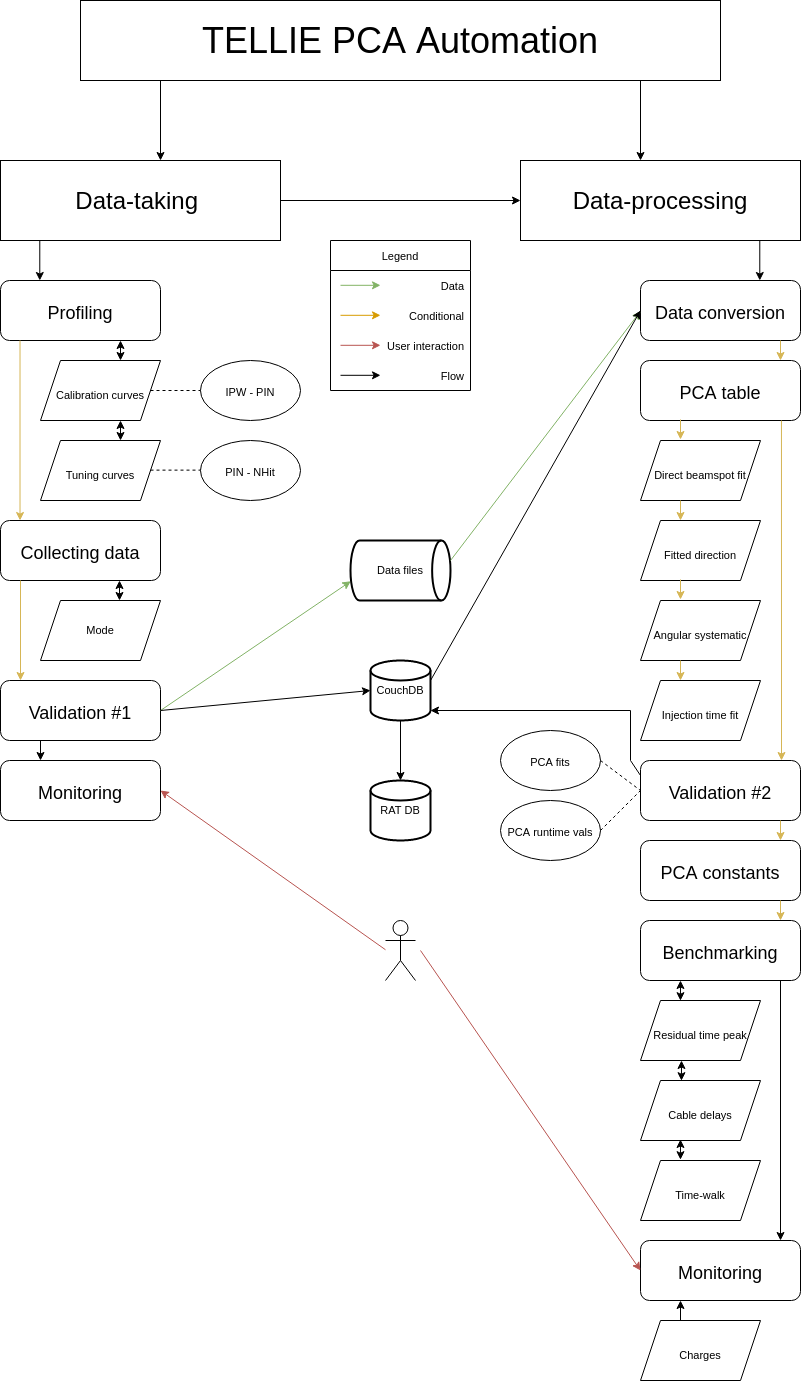
\includegraphics[width=0.37\textwidth]{plots/overview.png}}
\end{frame}

\begin{frame}{Validation \#1}
\textbf{Goal}: ensure that the data (just taken) is valid and can be used for PCA. 
\end{frame}

\begin{frame}{Validation \#1: correct fibre}
\noindent\makebox[\textwidth]{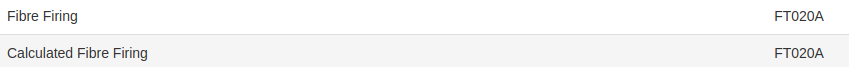
\includegraphics[width=1\textwidth]{plots/val1/cfib.png}}
\end{frame}

\begin{frame}{Validation \#1: Stats - events}
\noindent\makebox[\textwidth]{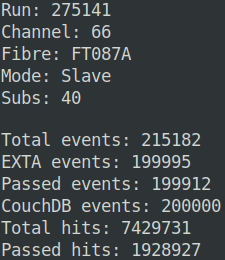
\includegraphics[width=0.37\textwidth]{plots/val1/stats.png}}
\center (missing EXTA recovery ?)
\end{frame}

\begin{frame}{Validation \#1: Stats - cuts}
\noindent\makebox[\textwidth]{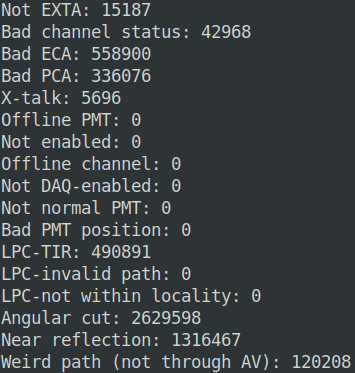
\includegraphics[width=0.37\textwidth]{plots/val1/cuts.png}}
\center threshold on valid events / hits
\end{frame}

\begin{frame}{Validation \#1: NHit}
\begin{minipage}{0.5\textwidth}
\noindent\makebox[\textwidth]{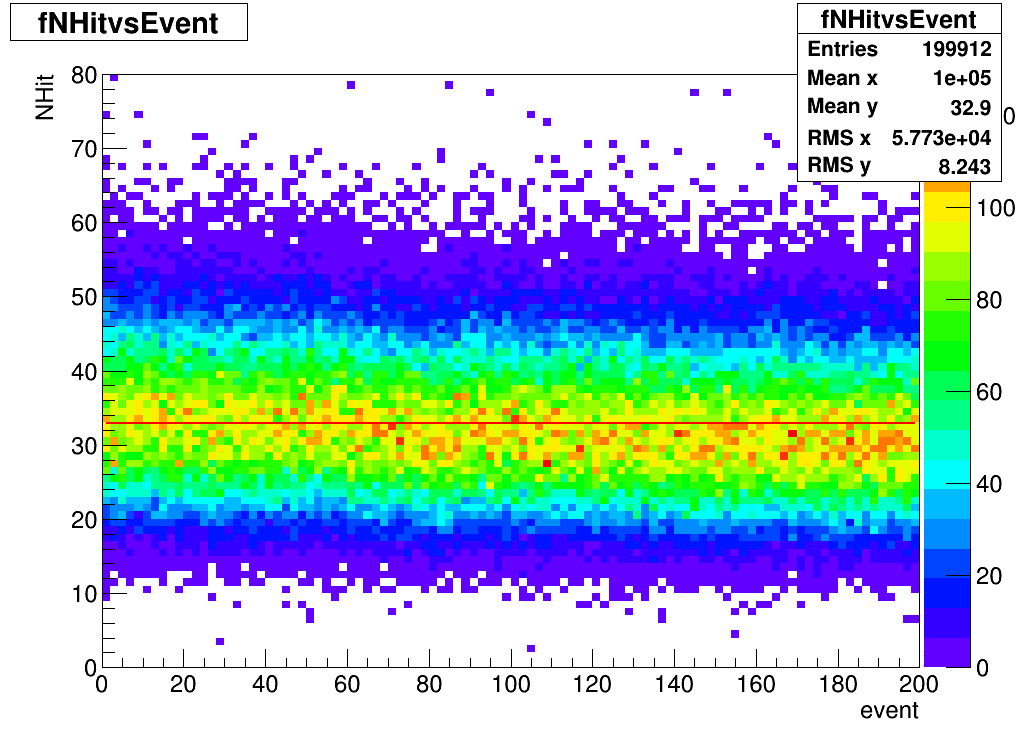
\includegraphics[width=1\textwidth]{plots/val1/nhittime.png}}
\end{minipage}%
\begin{minipage}{0.5\textwidth}
\noindent\makebox[\textwidth]{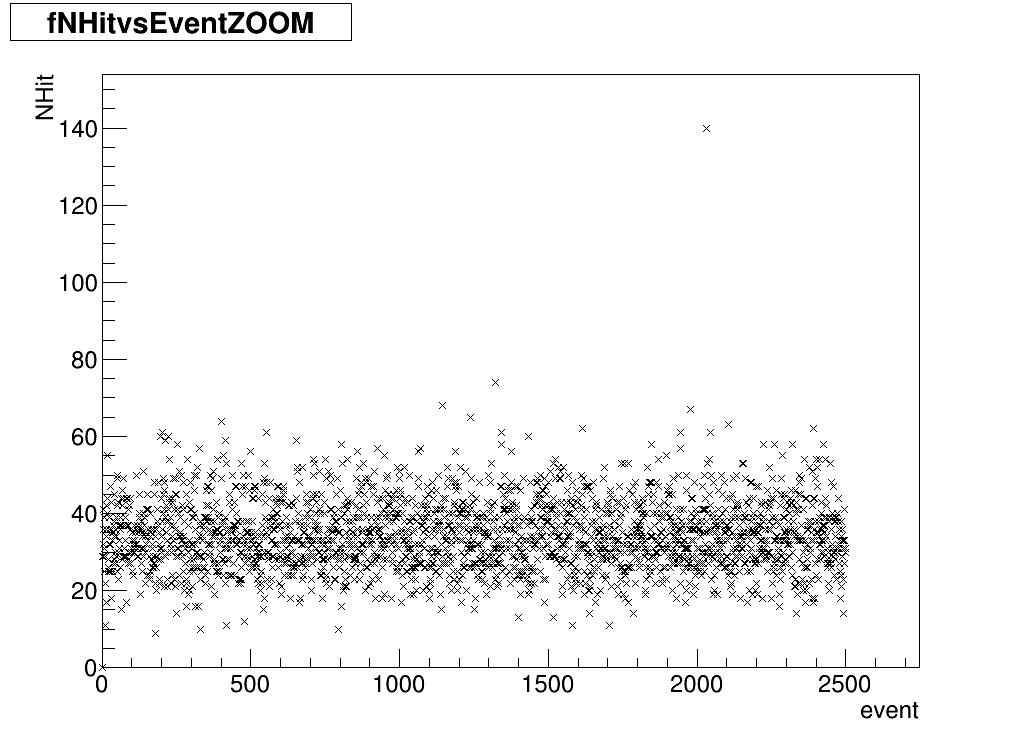
\includegraphics[width=1\textwidth]{plots/val1/nhitzoom.png}}
\end{minipage}
\center fibre intensity, stability
\end{frame}

\begin{frame}{Validation \#1: NHit}
\begin{minipage}{0.5\textwidth}
\noindent\makebox[\textwidth]{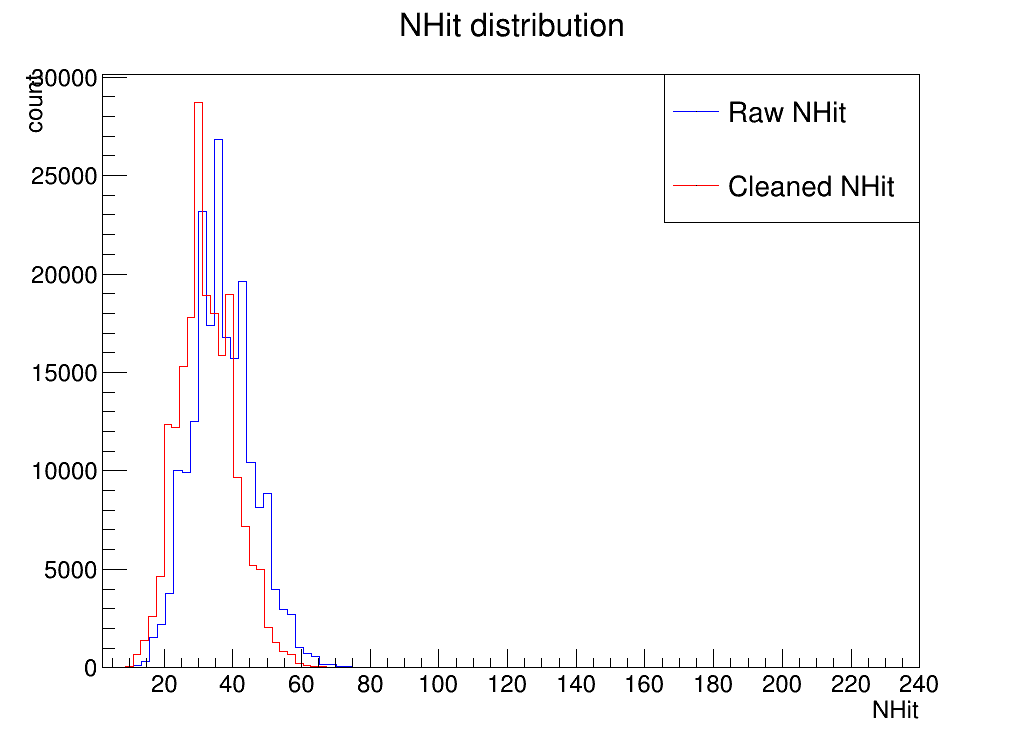
\includegraphics[width=1\textwidth]{plots/val1/nhitd.png}}
\center Raw
\end{minipage}%
\begin{minipage}{0.5\textwidth}
\noindent\makebox[\textwidth]{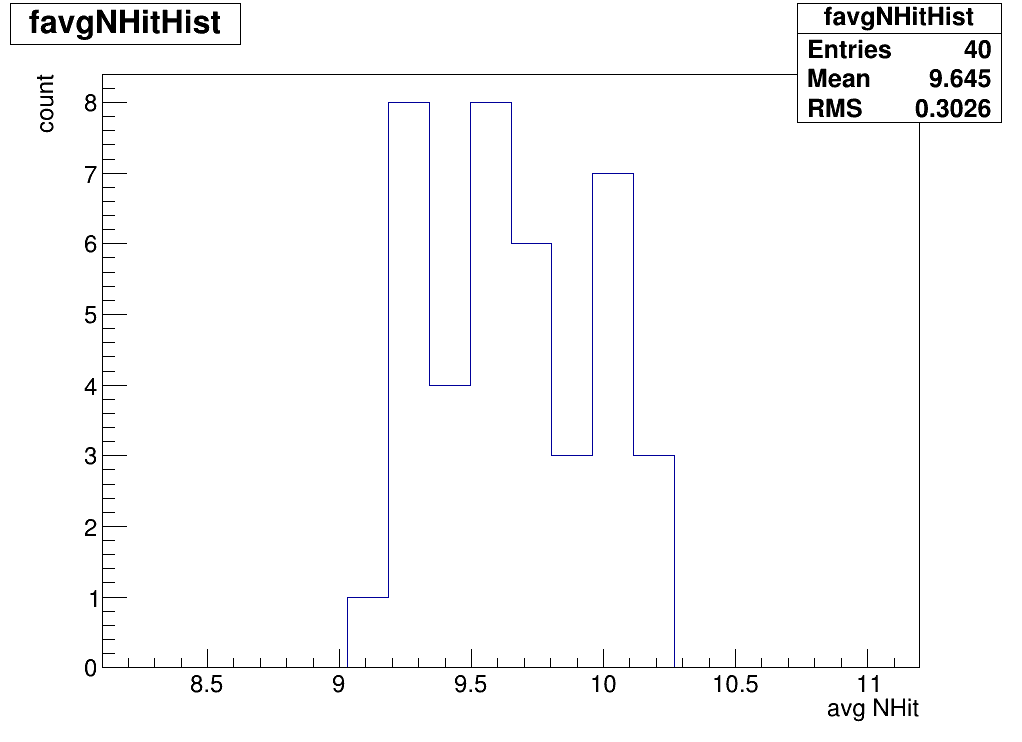
\includegraphics[width=0.75\textwidth]{plots/val1/avgN.png}}
\noindent\makebox[\textwidth]{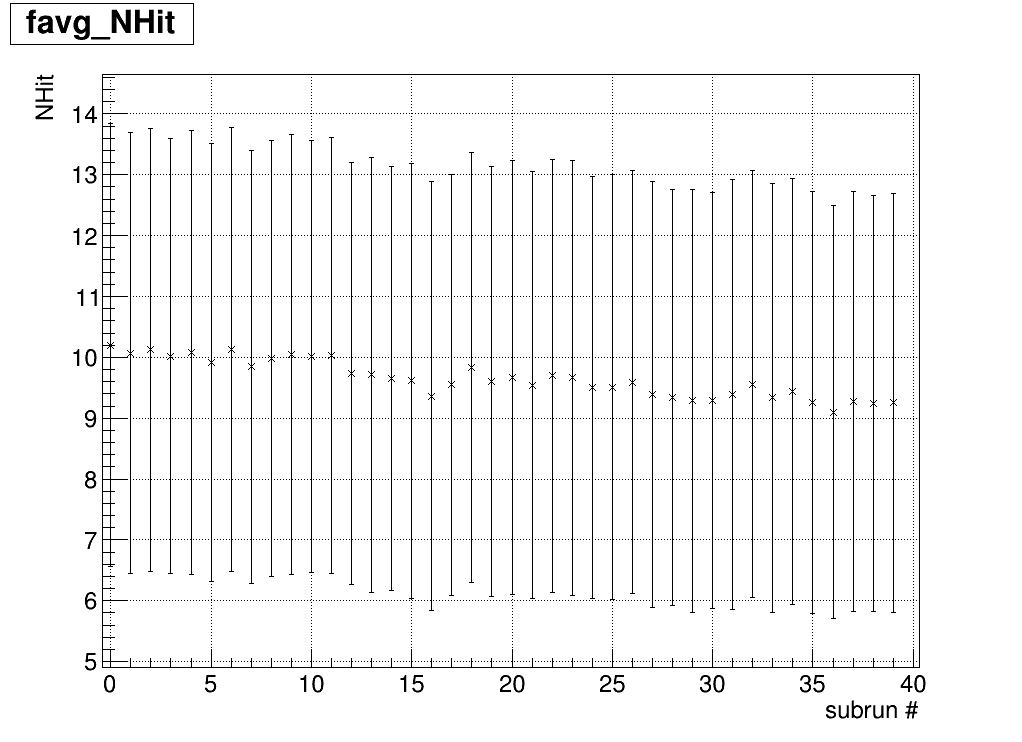
\includegraphics[width=0.75\textwidth]{plots/val1/avgNx.png}}
\center Valid hits
\end{minipage}
\end{frame}

\begin{frame}{Validation \#1: Occupancy}
\noindent\makebox[\textwidth]{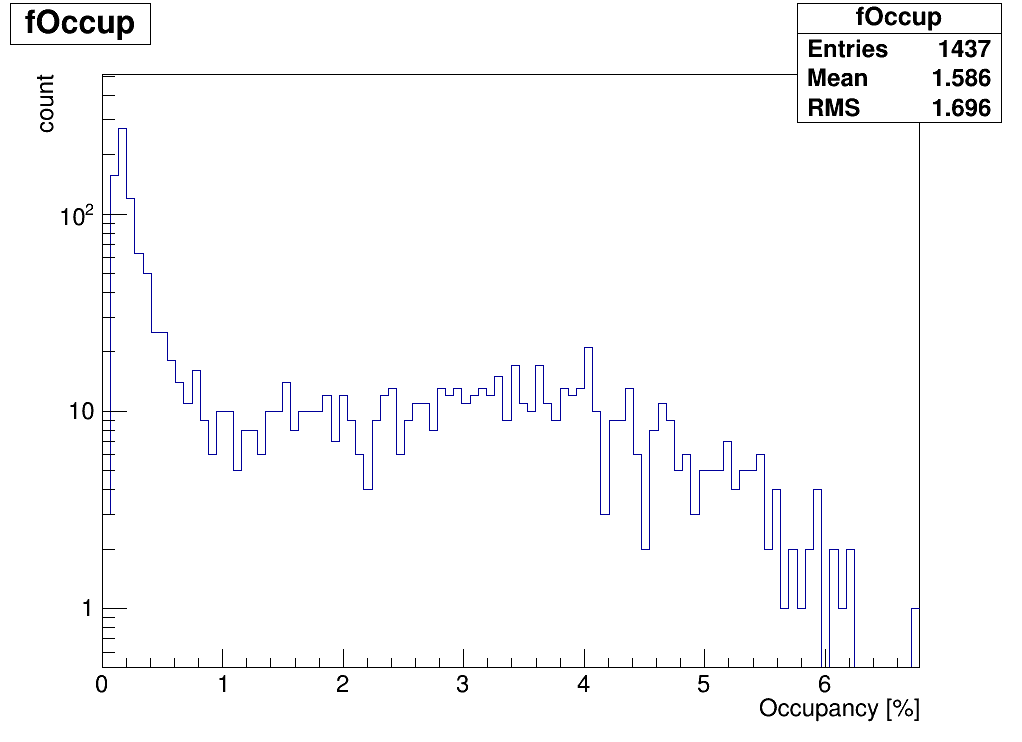
\includegraphics[width=0.38\textwidth]{plots/val1/o1.png}
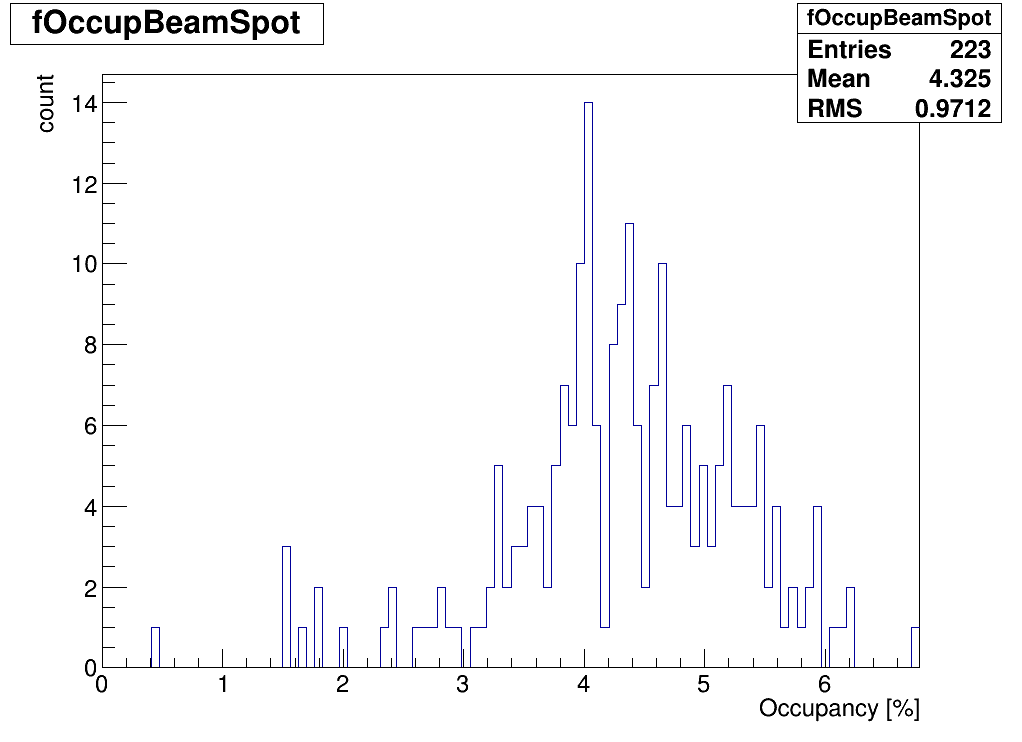
\includegraphics[width=0.38\textwidth]{plots/val1/o2.png}
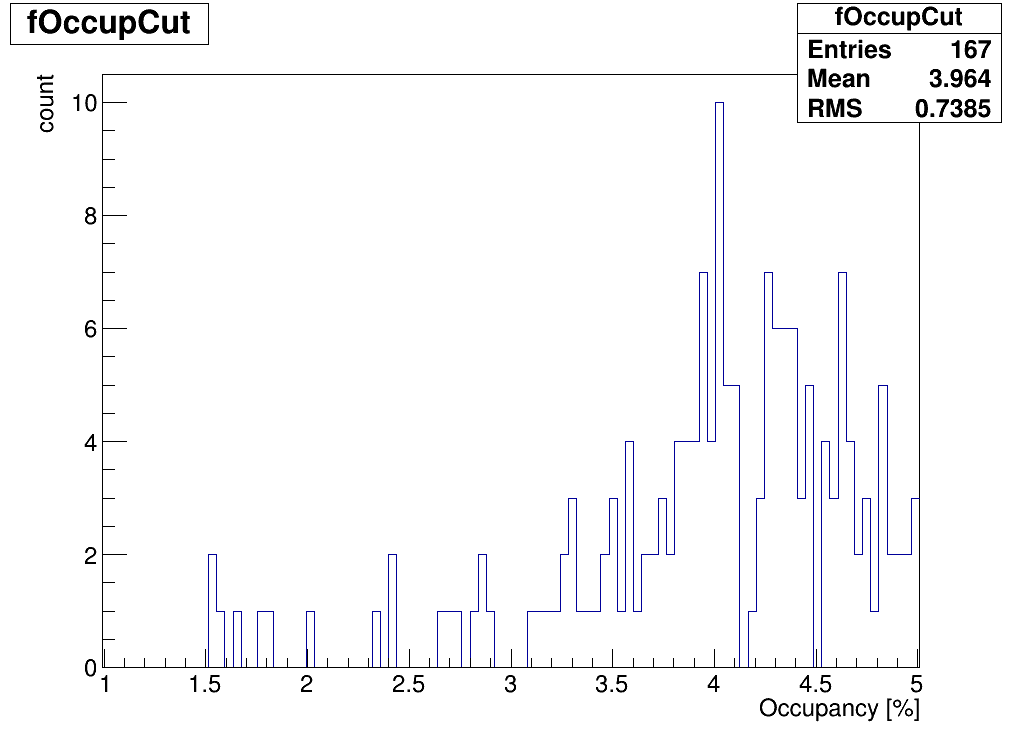
\includegraphics[width=0.38\textwidth]{plots/val1/o3.png}}
\center All \hfill Beamspot \hfill Cuts
\end{frame}

\begin{frame}{Validation \#1: Delays}
\begin{minipage}{0.5\textwidth}
\noindent\makebox[\textwidth]{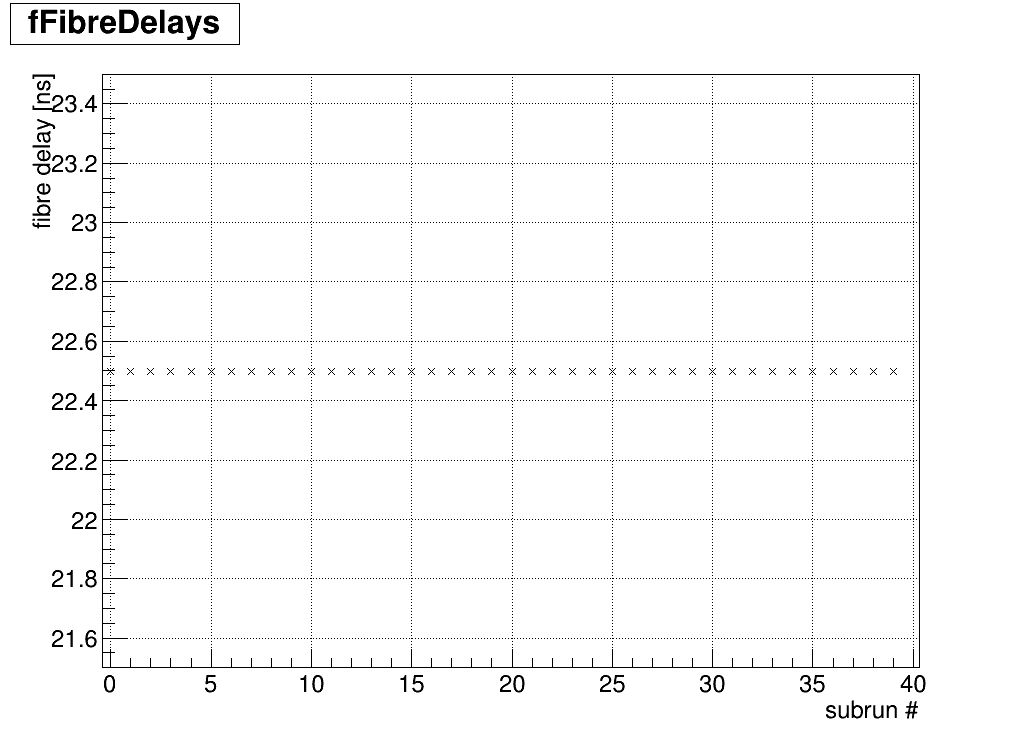
\includegraphics[width=1\textwidth]{plots/val1/fibd.png}}
\center Fibre delay
\end{minipage}%
\begin{minipage}{0.5\textwidth}
\noindent\makebox[\textwidth]{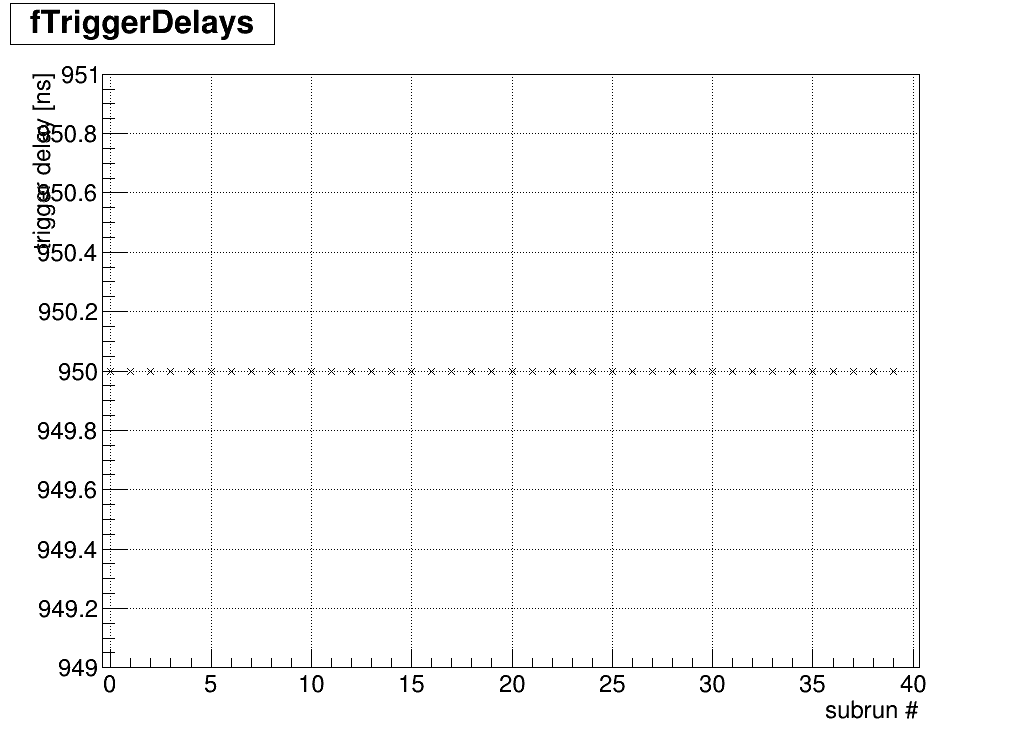
\includegraphics[width=1\textwidth]{plots/val1/trigd.png}}
\center Trigger delay
\end{minipage}
\end{frame}

\begin{frame}{Validation \#1: Time distribution}
\noindent\makebox[\textwidth]{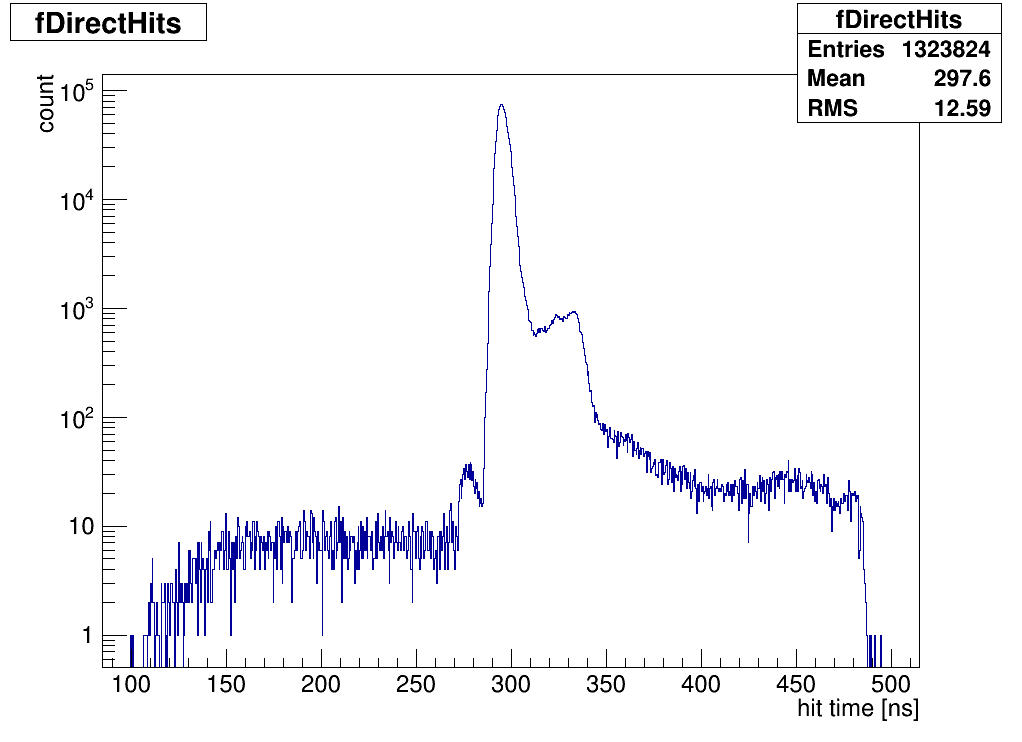
\includegraphics[width=0.38\textwidth]{plots/val1/times.png}
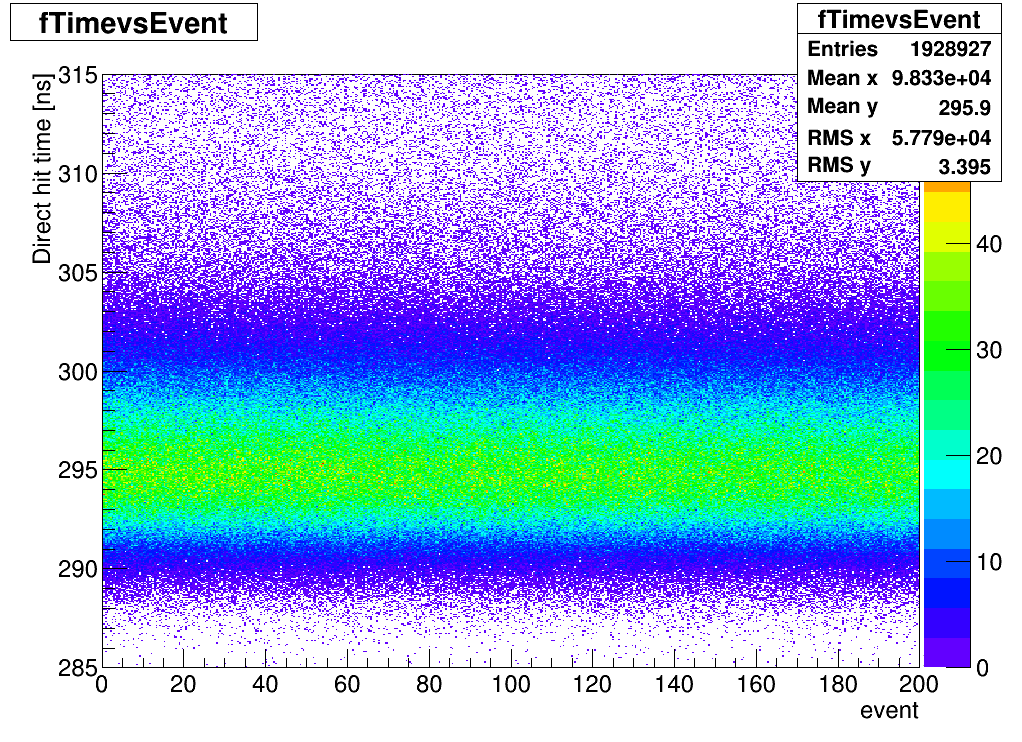
\includegraphics[width=0.38\textwidth]{plots/val1/timeev.png}
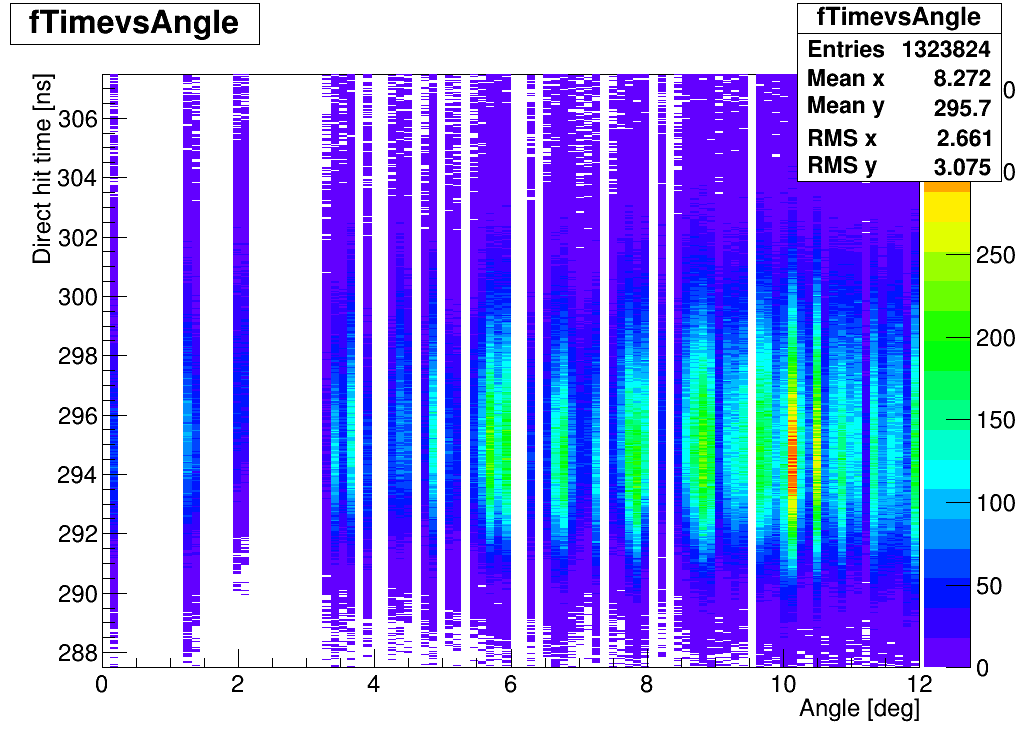
\includegraphics[width=0.38\textwidth]{plots/val1/timeangle.png}}
\center Direct hit time dist | \hfill Direct hit time f. evs | \hfill Direct hit time f. angle
\end{frame}

\begin{frame}{Validation \#1: PIN}
\noindent\makebox[\textwidth]{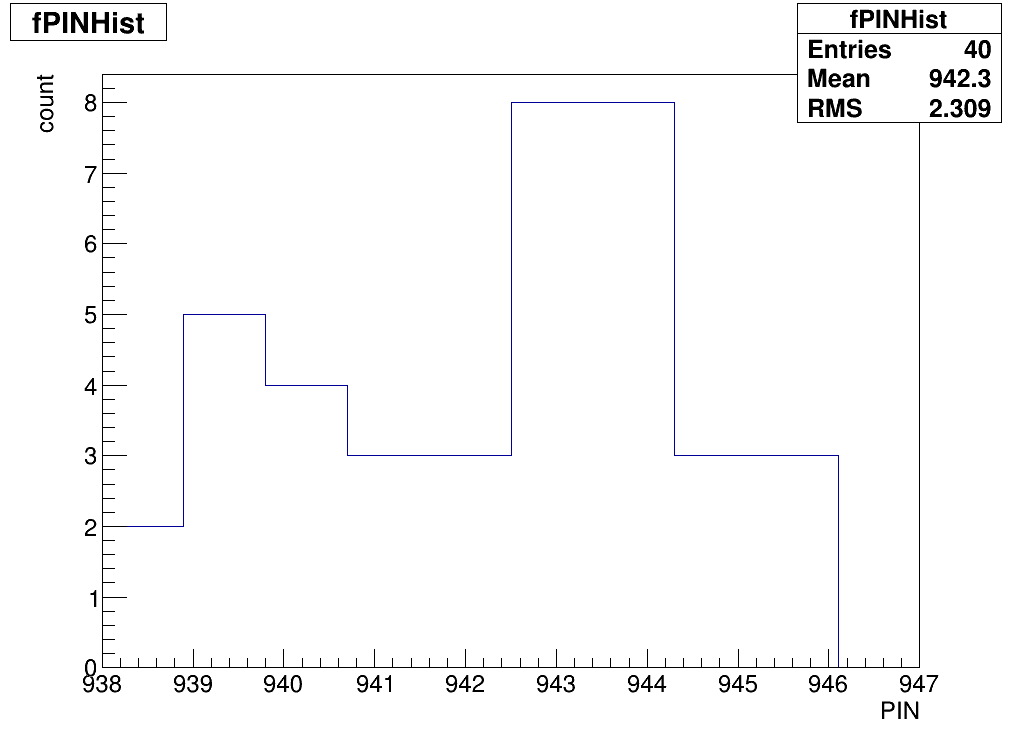
\includegraphics[width=0.38\textwidth]{plots/val1/pinH.png}
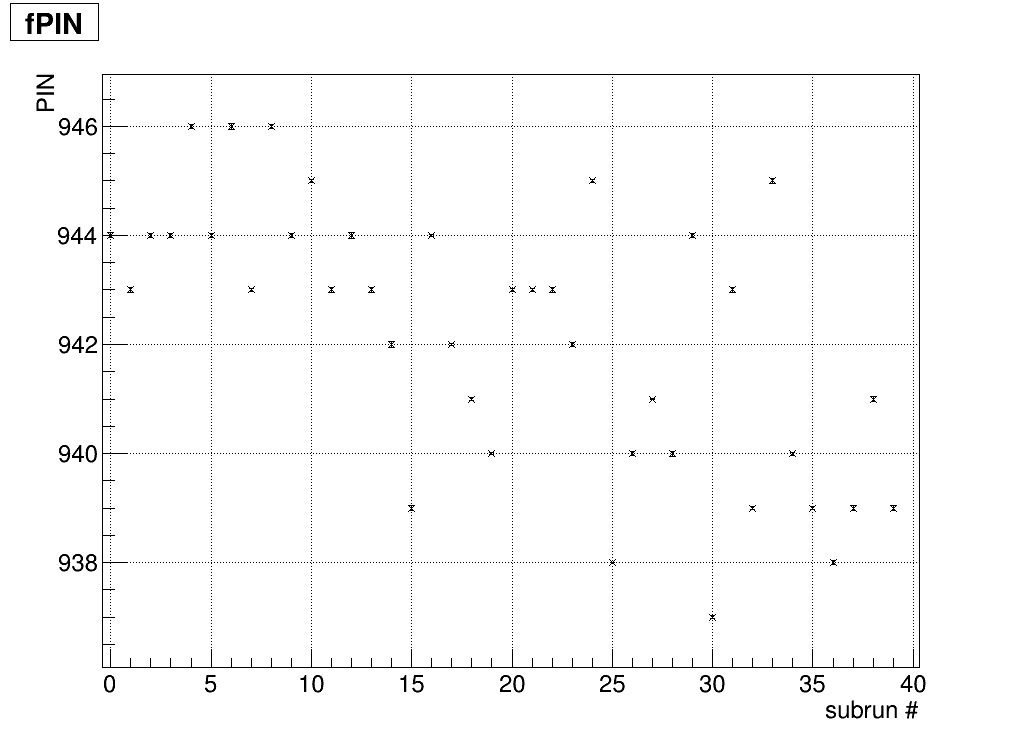
\includegraphics[width=0.38\textwidth]{plots/val1/pinx.png}
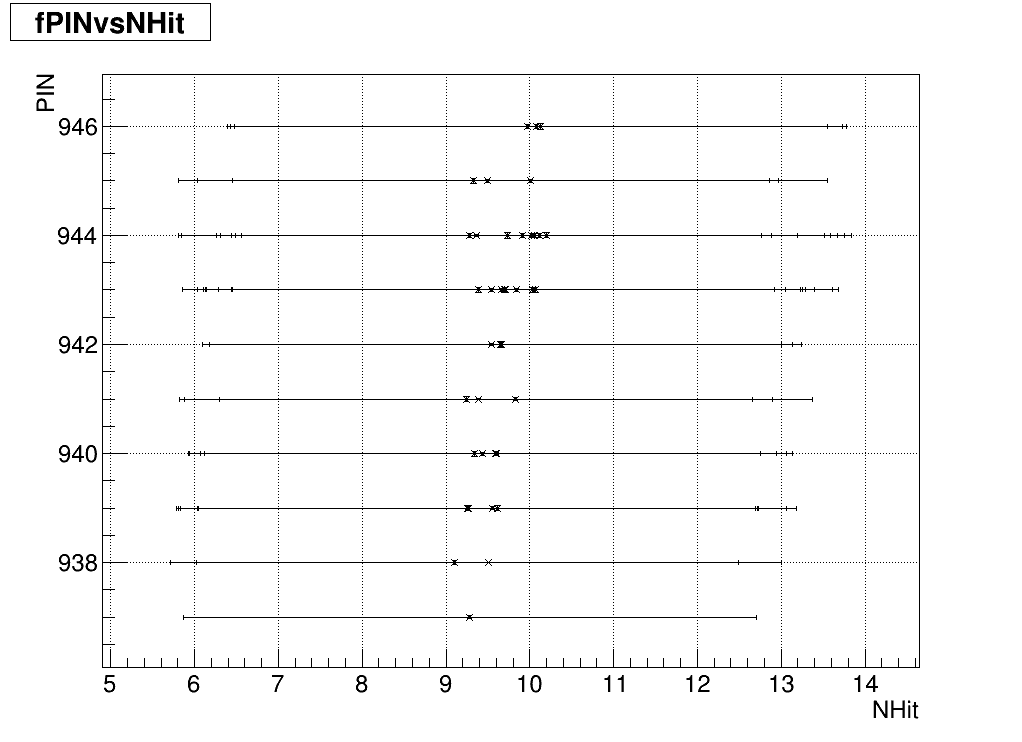
\includegraphics[width=0.38\textwidth]{plots/val1/PINNhi.png}}
\center PIN to NHit (tuning)
\end{frame}

\begin{frame}{Validation \#1: Angles}
\begin{minipage}{0.5\textwidth}
\noindent\makebox[\textwidth]{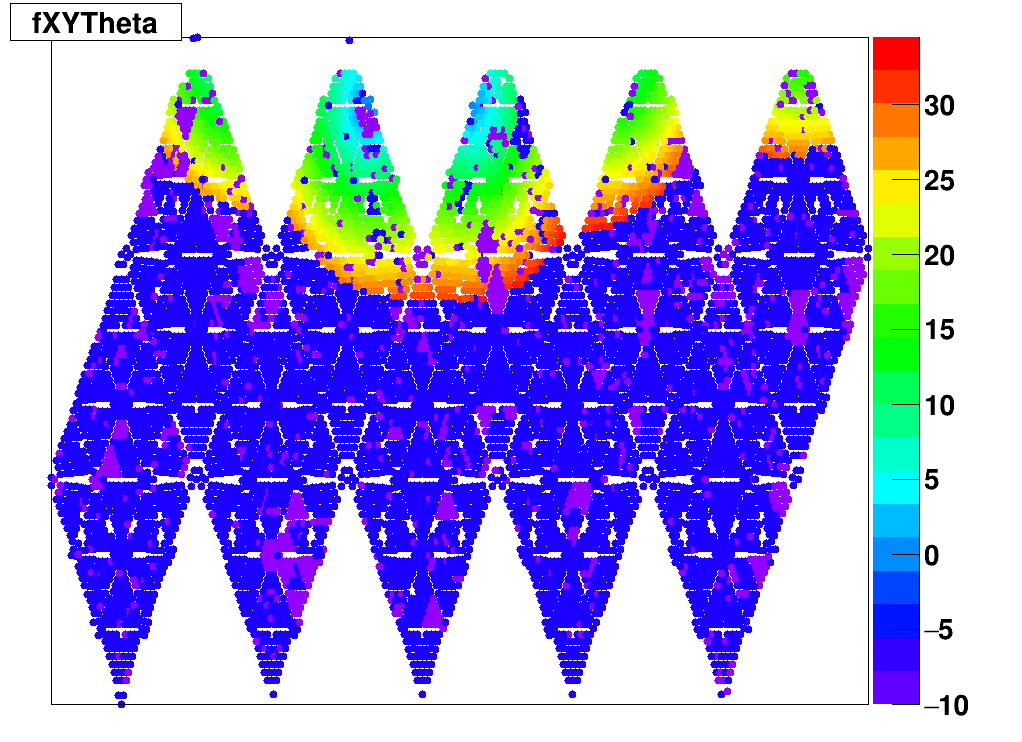
\includegraphics[width=1\textwidth]{plots/val1/thetaXY.png}}
\center angle: fibre - PMT
\end{minipage}%
\begin{minipage}{0.5\textwidth}
\noindent\makebox[\textwidth]{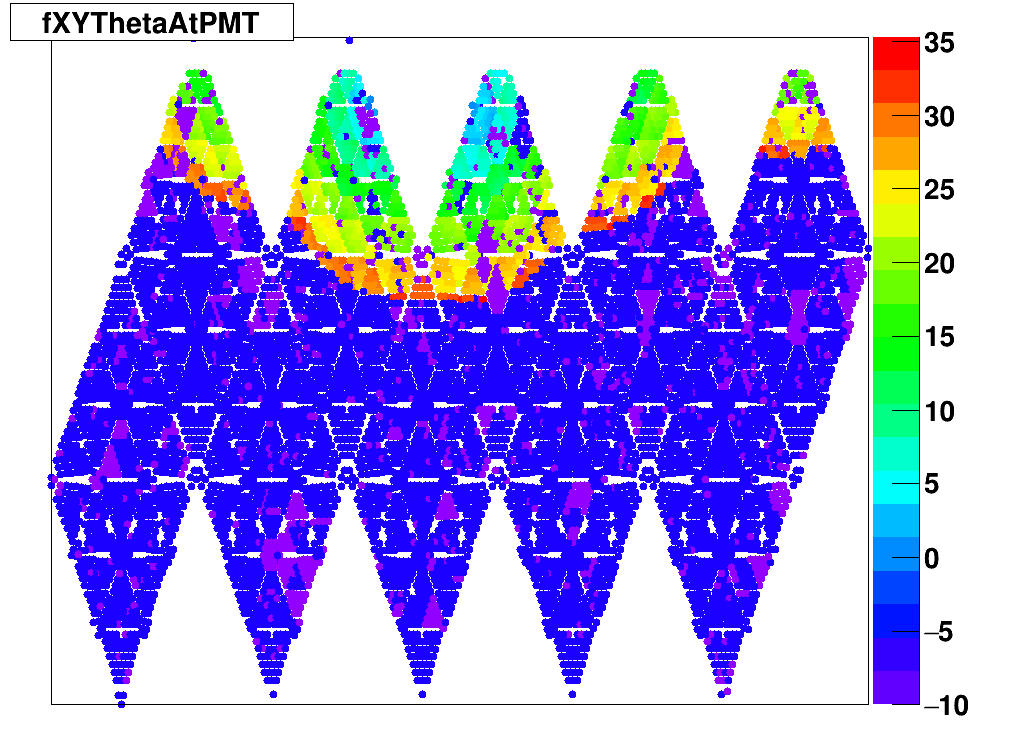
\includegraphics[width=1\textwidth]{plots/val1/thetaPMT.png}}
\center angle: light - PMT bucket
\end{minipage}
\center Some PMTs don't see light that should - DB with problematic PMTs?
\end{frame}

\begin{frame}{Validation \#1: More flat maps}
\begin{minipage}{0.5\textwidth}
\noindent\makebox[\textwidth]{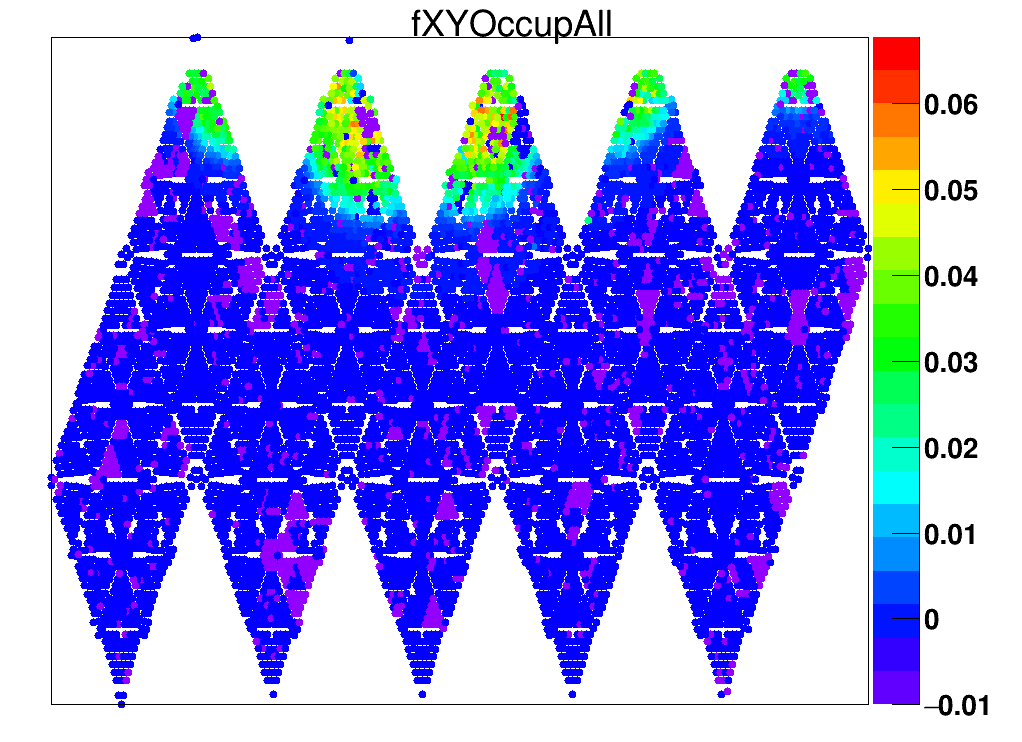
\includegraphics[width=1\textwidth]{plots/val1/occupXY.png}}
\center Occupancy (all)
\end{minipage}%
\begin{minipage}{0.5\textwidth}
\noindent\makebox[\textwidth]{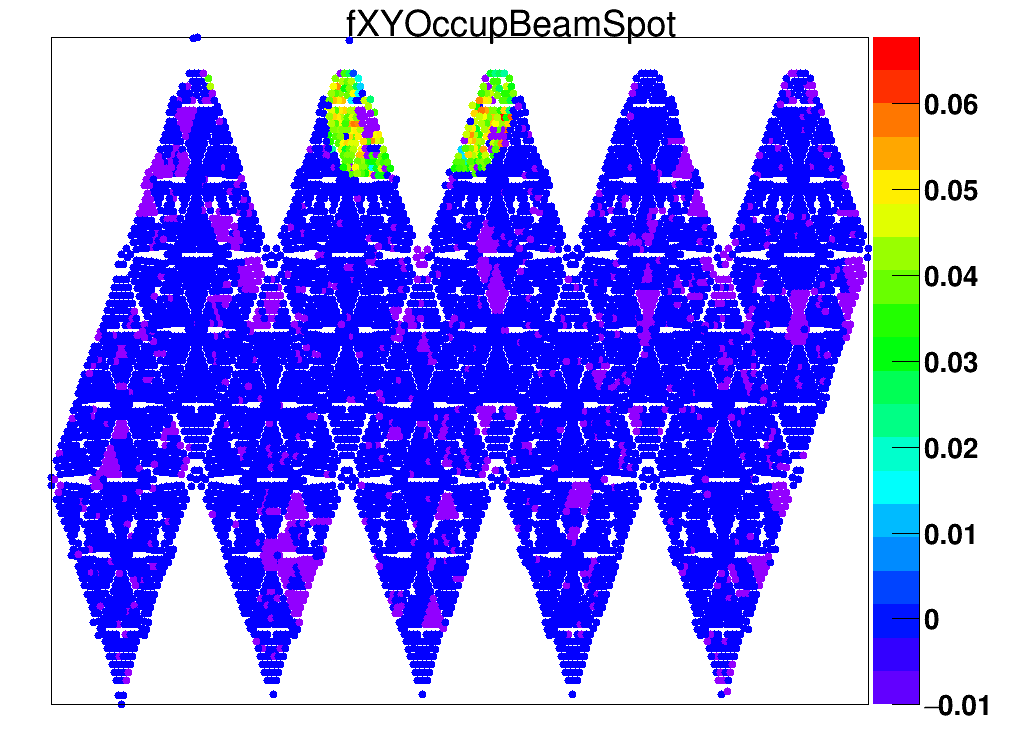
\includegraphics[width=1\textwidth]{plots/val1/occupbeam.png}}
\center Occupancy (beamspot)
\end{minipage}
\end{frame}

\begin{frame}{Validation \#1}
\textbf{Work}: need checks/thresholds based on the plots above to flag run good/bad. \\
If bad - retry. \\
If bad repeatedly - skip.
\end{frame}

\begin{frame}{PCA table}
\textbf{Goal}: fit for parameters required for the extraction of PCA constants.
\end{frame}

\begin{frame}{PCA table: Beam spot + direction}
\textbf{Goal}: fit the direct light beamspot, extract the direction from the fibre position (assume correct from DB), to the center of the beamspot.  \\
The process is based on splitting PMTs into faces (triangles) and fitting based on hits.\\
May be improved using dynamic beamspot / NHit instead.
\end{frame}

\begin{frame}{PCA table: Beam spot + direction}
\noindent\makebox[\textwidth]{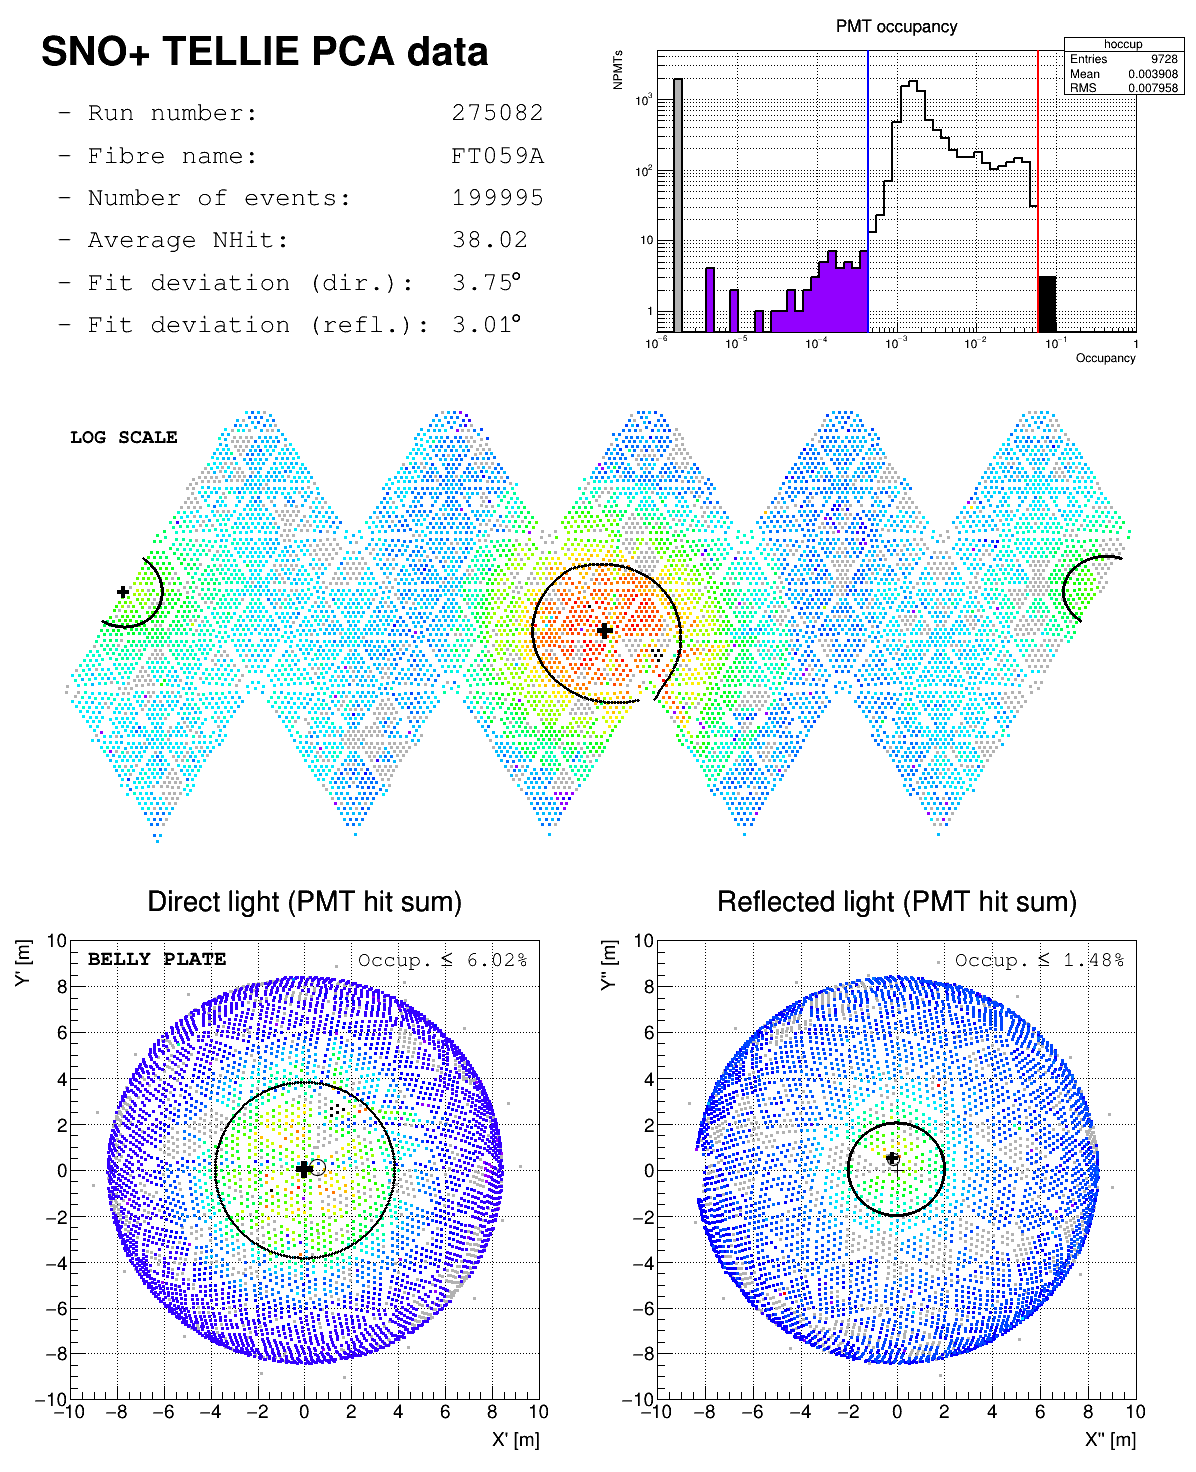
\includegraphics[width=0.55\textwidth]{plots/FT059A.png}}
\end{frame}

\begin{frame}{PCA table: Angular systematic}
\textbf{Goal}: evaluate the effect of modal dispersion for each fibre. Fit the distribution.\\
The angular range is wider here, since the effect is more pronounced at higher angles.\\
Requires previous PCA constants.
\end{frame}

\begin{frame}{PCA table: Angular systematic} 
\noindent\makebox[\textwidth]{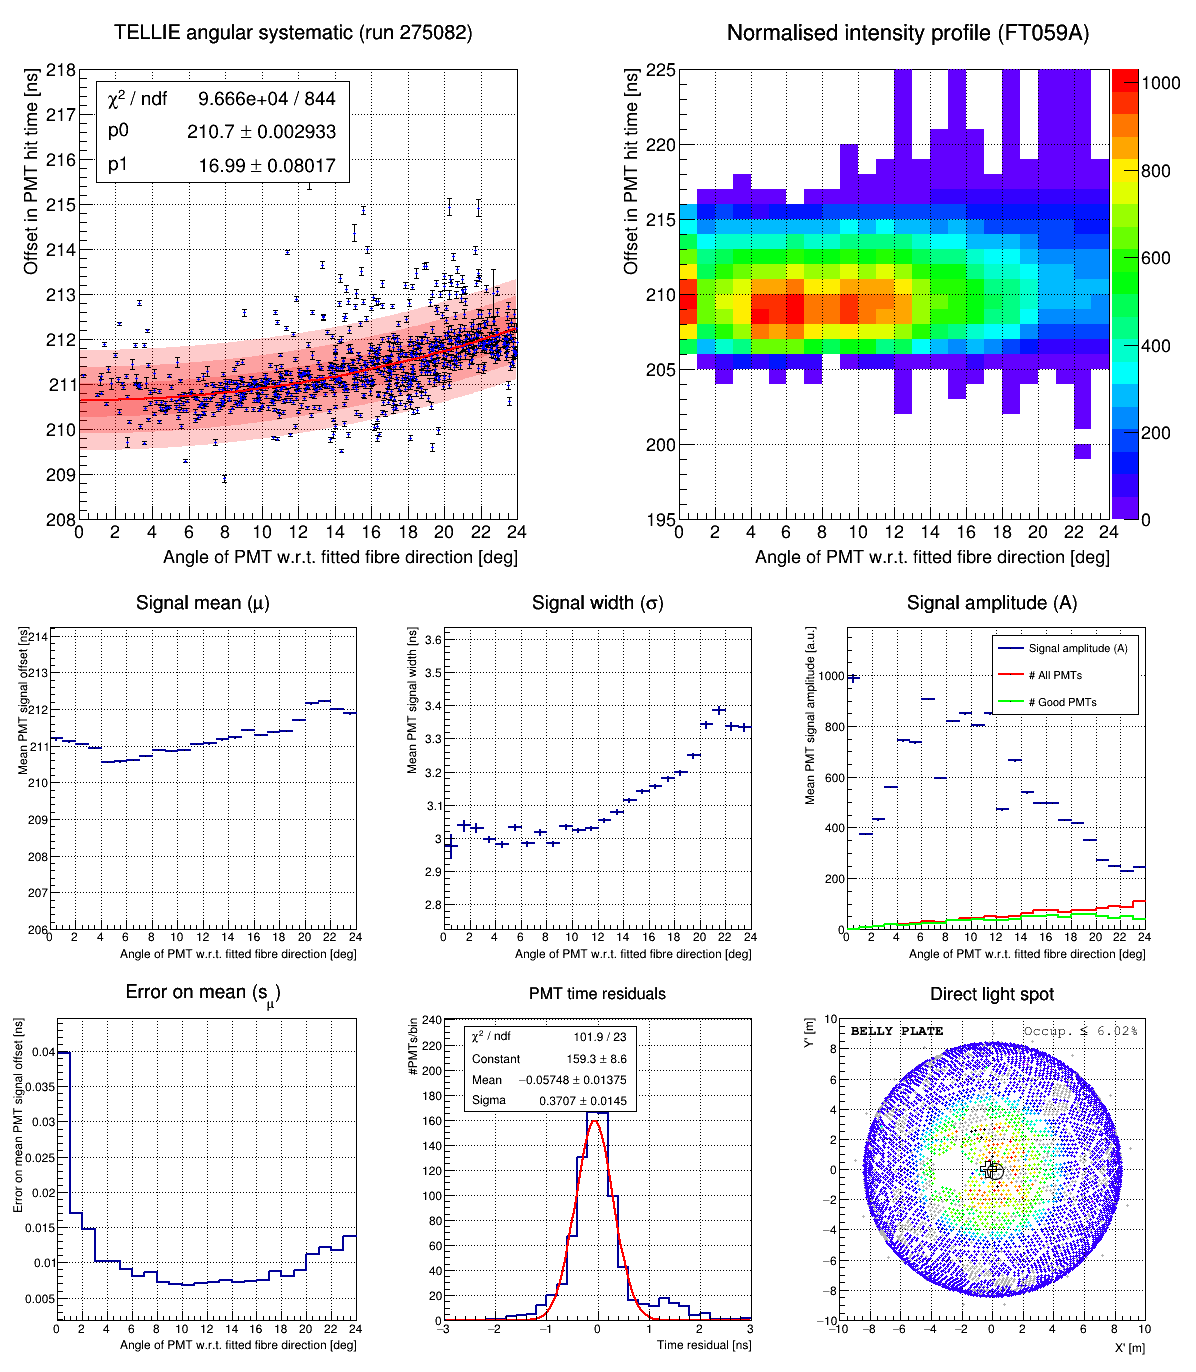
\includegraphics[width=0.58\textwidth]{plots/angular_FT059A.png}}
\end{frame}

\begin{frame}{PCA table: Injection time}
\textbf{Goal}: fit the injection time = \newline (hit time - bucket time - flight time - angular correction).\\Needed for PCA extraction.\\
Requires previous PCA constants
\end{frame}

\begin{frame}{PCA table: Angular systematic} 
\noindent\makebox[\textwidth]{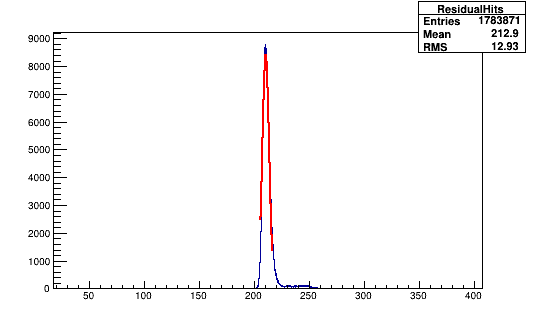
\includegraphics[width=0.58\textwidth]{plots/1.png}
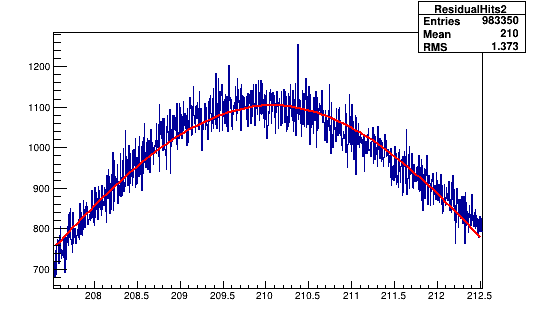
\includegraphics[width=0.58\textwidth]{plots/2.png}}
\end{frame}

\begin{frame}{Validation \#2}
\textbf{Goal}: check new pca table values - reasonable? Compare to previous set(s).
Will include:
\begin{itemize}
	\item Time of flight correction
	\item Bucket time correction
	\item Angular systematic correction
	\item Fibre direction deviation
	\item Emission time
	\item Run-time values: IPW, delays...
\end{itemize}
\end{frame}

\begin{frame}{PCA constants}
\textbf{Goal}: PCAProc that extracts the PCA values. \\
Idea: split LB and TELLIE processor. \\
(LB processor not used/tested for scintillator.)
\end{frame}

\begin{frame}{Monitoring}
\textbf{Goal}: revive old PCA monitoring page.
\noindent\makebox[\textwidth]{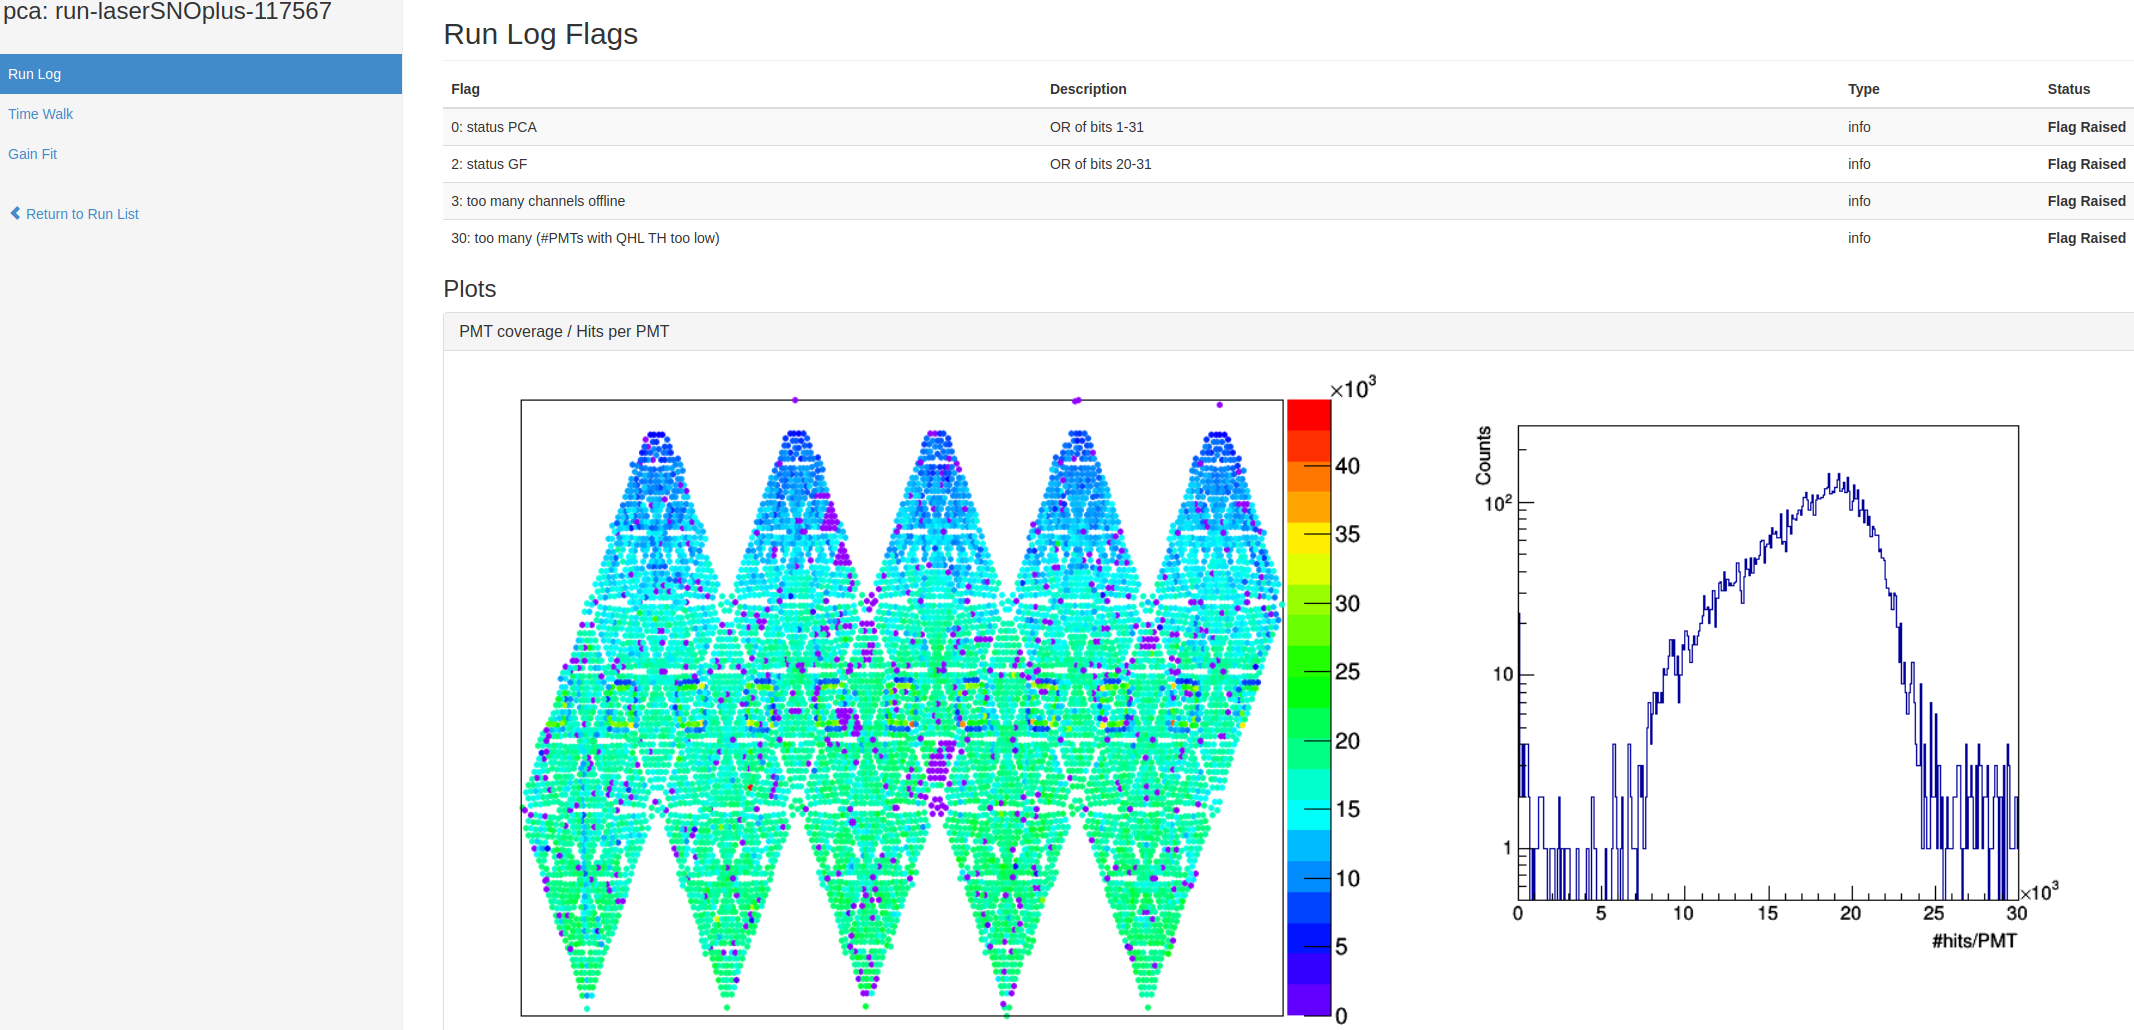
\includegraphics[width=1\textwidth]{plots/mon.png}}
\end{frame}

\begin{frame}{Open questions}
\begin{itemize}
	\item tagging of events outside Orca
	\item when (from) to apply new constants
	\item DB with electronic issues for PMTs
	\item ensure recent ECA
	\item discrete vs continuous mode
	\item continuous data-taking: run-type changes, run rollovers, breakdowns...
	\item data conversion - now not needed
	\item server to run this on, with access to data (snug1 / snug2)
	\item unified event selection, hit cuts
\end{itemize}
\end{frame}

\begin{frame}{List of cuts: EXTA}
EXTA event (macro):
\begin{tcolorbox}
/rat/proc/if trigTypeSelector
  \# None of the following
  \hspace*{5mm} /rat/procset trigType "N100Low" \\
  \hspace*{5mm} /rat/procset trigType "N100Med" \\
  \hspace*{5mm} /rat/procset trigType "N100High" \\
  \hspace*{5mm} /rat/procset trigType "N20" \\
  \hspace*{5mm} /rat/procset trigType "N20LB" \\
  \hspace*{5mm} /rat/procset trigType "Pedestal" \\
  \hspace*{5mm} /rat/procset trigType "EXT8PulseAsy" \\
/rat/proc/else \\
  \hspace*{5mm} /rat/proc/if trigTypeSelector \\
  \hspace*{5mm}\hspace*{5mm}  \#Only pure EXTA \\
  \hspace*{5mm}\hspace*{5mm} /rat/procset trigType "EXTASY"
\end{tcolorbox}
\end{frame}

\begin{frame}{List of cuts: EXTA}
EXTA event (code):
\begin{tcolorbox}
trig = ev.GetTrigType(); \\ 
if (!(trig \& 0x8000))
\end{tcolorbox}
\end{frame}

\begin{frame}{List of cuts: PMTs}
\begin{tcolorbox}
const RAT::DS::CalPMTs\& pmts = ev.GetCalPMTs(); \\
for(int iPMT=0;iPMT<pmts.GetNormalCount();iPMT++)\{\\
RAT::DS::PMTCal pmt = pmts.GetNormalPMT(iPMT); \\
int pmtID = pmt.GetID(); \\
const RAT::DU::PMTCalStatus\& pmtStatus = RAT::DU::Utility::Get()->GetPMTCalStatus(); \\
const RAT::DU::ChanHWStatus\& chs = RAT::DU::Utility::Get()->GetChanHWStatus(); \\
const RAT::DU::PMTInfo\& pmtinfo\_loop = RAT::DU::Utility::Get()->GetPMTInfo();
\end{tcolorbox}
\end{frame}

\begin{frame}{List of cuts: PMTs}
\begin{tcolorbox}
unsigned int status = pmtStatus.GetHitStatus(pmt);\\
if(status \& (1<<pmtStatus.kCHSBit))\{continue;\}\\
if(status \& (1<<pmtStatus.kECABit))\{continue;\}\\
if(status \& (1<<pmtStatus.kPCABit))\{continue;\}\\
if(status \& (1<<pmtStatus.kXTalkBit))\{continue;\}\\
if ( !chs.IsTubeOnline(pmtID) )\{continue;\}\\
if ( !chs.IsEnabled() )\{continue;\}\\
if ( !chs.IsChannelOnline(pmtID) )\{continue;\}\\
if ( !chs.IsDAQEnabled(pmtID) )\{continue;\}\\
if ( pmtinfo\_loop.GetType(pmtID) != 1 )\{continue;\}
\end{tcolorbox}
\center (chs cuts are also used to mark offline PMTs)
\end{frame}

\begin{frame}{List of cuts: PMTs}
\begin{tcolorbox}
const RAT::DU::PMTInfo\& pmtinfo = RAT::DU::Utility::Get()->GetPMTInfo();\\
TVector3 pmtPos = pmtinfo.GetPosition(pmtID);\\
if (pmtPos.Mag()==0)\{continue;\} 
\end{tcolorbox}
\end{frame}

\begin{frame}{List of cuts: LPC}
\begin{tcolorbox}
RAT::DU::LightPathCalculator lpc = RAT::DU::Utility::Get()->GetLightPathCalculator();\\
lpc.SetELLIEEvent(true);\\
lpc.CalcByPosition(fibrepos, pmtPos, energy, LOCALITY);\\
if (lpc.GetTIR() == 1) \{continue;\}\\
if (lpc.GetPathValid() == 0) \{continue;\}\\
if (lpc.GetResvHit() == 1) \{continue;\}  \\  \\
if (lpc.GetTotalDist() <= 12000)\{continue;\}\\
if (lpc.GetDistInInnerAV() <= 9000)\{continue;\}\\ \\
if ( (theta > 12) || (theta < 0) ) \{continue;\}
\end{tcolorbox}
\end{frame}

\begin{frame}{List of cuts: Occupancy}
\begin{tcolorbox}
pmtOccup[iPMT] = (float)fPMTs[iPMT][7][0]/(float)allEvs;\\
if ( pmtOccup[iPMT] >= 0.01 \&\& pmtOccup[iPMT] <= 0.05)\{...\}
\end{tcolorbox}
\end{frame}

\end{document}